% jeg vil starte med at lave en meget rodet kladde som indeholder en masse ideer. Og så rydde langsomt op i den.


% 15 * 2400 = 36000 anslag


\documentclass[
%journal=ancac3, % for ACS Nano
%journal=acbcct, % for ACS Chem. Biol.
journal=jacsat, % for undefined journal
manuscript=article]{achemso}



\usepackage[utf8]{inputenc}
\usepackage{blindtext}
%\usepackage{showframe}
%\usepackage{lmodern}

%\renewcommand*\familydefault{\sfdefault} 


% https://tex.stackexchange.com/questions/121061/working-with-arial-or-helvetica-fonts#121063
%\usepackage[scaled]{helvet}
%\renewcommand\familydefault{\sfdefault} 
%\usepackage[T1]{fontenc}


\usepackage[scaled=1]{tgheros}
\usepackage[helvet]{sfmath}
\renewcommand{\familydefault}{\sfdefault}
\everymath={\sf}
\usepackage[T1]{fontenc}



%\usepackage[T1]{fontenc}
%\usepackage{lmodern}
%\usepackage[version=3]{mhchem} % Formula subscripts using \ce{}

%\newcommand*{\mycommand}[1]{\texttt{\emph{#1}}}


\author{Carl Mathias Kobel}

\affiliation{BiRC, AU}

\email{kobel@pm.me}

\title[\texttt{achemso} demonstration]
{Bachelor internship: Copy Number Variation of Ampliconic Regions on Hominid X and Y chromosomes}

\begin{document}

\begin{abstract}
As we are interested in describing the ampliconic genes on the hominid X chromosome, we assembled species specific artificial chromosomes containing orthologs of genes which are known to be ampliconic in human. By mapping reads from several chimpanzee and gorilla individuals upon these species specific artificial chromosomes, we measured the copy number variation and showed that several of these genes might not be ampliconic in these human-related species.
\end{abstract}

%\clearpage
%%%%%%%%%%%%%%%%%%%%%%%%%%%%%%%%%%%%%%%%%%%%%%%%%%%%% Introduction
\section{Introduction}


\subsection{Sex determining systems} % Mostly content from Elise's master
% I want to start by introducing the sex determ. systems.
The sex determining system present (in mammals) today most probably arose because a variant on one of the homologous chromosomes disrupted the former sex determining system, which is supposed to have been environmental (i.e. temperature regulated as in some ). This is, according to Ohno's model (Ohno 1967) the explanation for the development of the ZW (heterogametic female) sex determining system. It has since been shown (with comparative mapping) that the development of the XY (heterogametic male) sex determining system most probably has a similar origin.
This variant may have been the start of the divergence between the sex chromosomes. The SRY gene (on the Y chromosome) is considered the Testis Determining Factor which means that the presence of this gene defines the sex of an individual (in mammals).

Although the sex chromosomes have diverged to become very different, they still have areas with recombination in the very ends called PAR1 and PAR2. These actively recombining areas are needed for successful cell division and are thus conserved from before the divergence.

%
Correlation between sexual behaviour and sperm quality. ??reference

\subsection{Ampliconic genes} % Mostly content from Elise's paper 17
Ampliconic genes are present only on sex chromosomes. They consist of very similar adjacent duplications with copy numbers anywhere between 2 and 40. The mechanism by which they duplicate is not known. Many ampliconic genes are testis expressed and assumed (??why) to be involved in in meiotic drive processes. Meiotic drive favours the segregation of specific genes, thus disturbing the mendelian segregation ratios. As the genetic homology between human and mouse is much higher for single copy genes, than for ampliconic genes, it is suggested that the evolutionary turnover is much faster for ampliconic genes. Ampliconic genes are suspected?? to be drivers of speciation, since a fast duplication mechanism may render the recombination of X chromosomes impossible ??speculation.


% overgang
As the copy number of ampliconic genes have already been described in human, we now want to investigate how many of these genes also show ampliconic behaviour in chimpanzee and gorilla.


%Citation of Einstein paper~\cite{doi:10.1093/molbev/msi198}.

\clearpage
%%%%%%%%%%%%%%%%%%%%%%%%%%%%%%%%%%%%%%%%%%%%%%%%%%%%% Method
\section{Method}

The pipeline\cite{cmkpipe} (Figure \ref{fig:pipeline}) of this project consists of several parts, all originating from \textit{Lucotte et al.\cite{LucotteDyn}}. Firstly, an artificial chromosome with ampliconic candidates was assembled for each species, for each of their sex chromosomes. Later, genome reads were mapped upon the artificial chromosome, and the copy number was estimated in relation to a non-ampliconic control.
%\def\code#1{\texttt{#1}}


\begin{figure}
  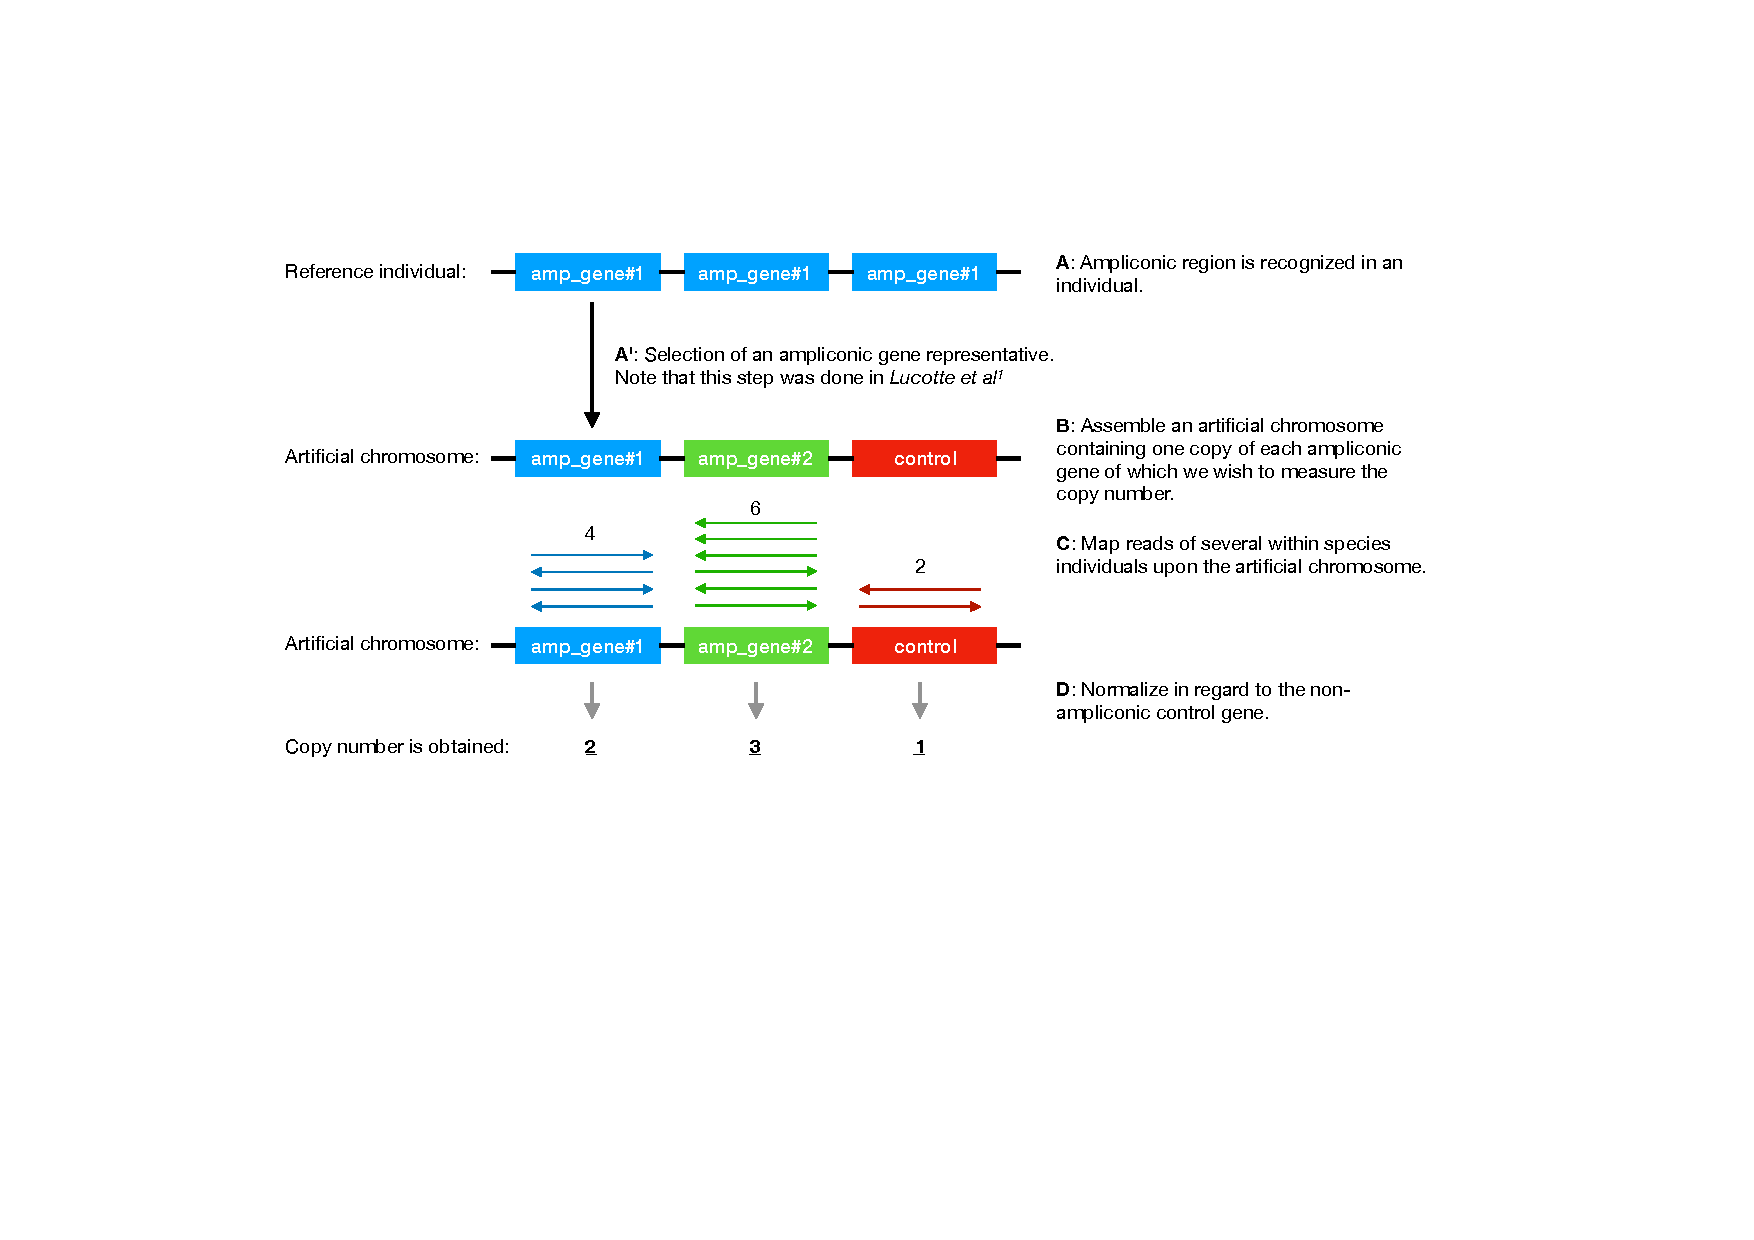
\includegraphics[width=\linewidth]{illustrations/figure_pipeline.pdf}
  \caption{A complete overview of the pipeline.}
  \label{fig:pipeline}
\end{figure}



\subsection{Assembly of artificial chromosome}
In order to assemble the artificial chromosomes we took inspiration from \textit{Lucotte et al.\cite{LucotteDyn}} and selected all the genes that exhibited an ampliconic nature. In this paper, the genes selected because they exhibited an ampliconic nature in dotplots. (?? Why is it that only such few genes are indeed ampliconic, if they look like they all should be on the dotplot??) We searched for orthologs in chimpanzee (reference: Pan\_tro\_3.0) and gorilla (reference: gorGor4) for the associated human genes (reference: GRCh38.p12) in the Ensembl genome browser. Only orthologs with a subject/query identical factor of more than 0.5 and a length of at least of the original (??) were included (see Table \ref{tab:orthologs}). When orthologs were not found in the Ensembl genome browser, we blasted the human genes against the chimpanzee and gorilla references \texttt{blastn -subject <reference>.fa -query <human\_gene>.fa -out output.txt} and again only selected regions with a subject/query identical factor of more than 0.5 and ortholog length divided by original length of at least 0.5 as well. The orthologs found on ensembl were downloaded directly as fasta files. The orthologs found with BLAST were cut out of the reference with SAMtools. The isolated genes were later merged into a complete artificial chromosomes with GNU cat. These artificial chromosomes (chimpanzee X, chimpanzee Y and gorilla X) were then put into the read-mapping pipeline presented in the next part. Several problems occured in the assembly of the artificial chromosomes. We checked coherence between Ensembl and BLAST results with GAGE4 in gorilla. The Query \%id and BLAST Identities are on par, but the length fraction is far off. This may be due to the way the human ampliconic regions were chosen. The human ampliconic regions from \textit{Lucotte et al.\cite{LucotteDyn}} has a length of 7330bp whereas the corresponding gene on Ensembl has a length of 15285bp. A supposed remedy is to blast the human genes from Ensembl against the chimpanzee and gorilla references. (?? this is surely because i have misunderstood something about the assembly of human ACs)



\begin{table}
\footnotesize
    \begin{center}
        \begin{tabular}{  l | c | l | p{1.8cm} | p{1.8cm} | p{1.8cm} | p{1.8cm} }
                \textbf{Species} & \textbf{Chr.} & \textbf{Gene} & \textbf{Ensemble Query id\%} & \textbf{Ensembl length fraction} & \textbf{BLAST Identities} & \textbf{BLAST length fraction} \\ 
                \hline
                    Chimpanzee & X & CT45A5 & 0.96 & 1.81 & - & - \\ 
                    Chimpanzee & X & CT47A4 & 0.92 & 1.15 & - & - \\ 
                    Chimpanzee & X & GAGE4 & 0.82 & 2.27 & - & - \\ 
                    Chimpanzee & X & OPN1LW & - & - & 0.98 & 0.95 \\ 
                    Chimpanzee & X & SPANXB1 & 0.68 & 0.85 & - & - \\ 
                    Chimpanzee & X & DMD (control) & 0.99 & 1.00 & - & - \\ 
                    \hline
                    Gorilla & X & CT45A5 & 0.78 & 0.76 & - & - \\ 
                    Gorilla & X & CT47A4 & 0.80 & 0.31 & - & - \\ 
                    Gorilla & X & GAGE4 & 0.89 & 2.09 & 0.90 & 0.51 \\ 
                    Gorilla & X & SPANXB1 & 0.67 & 1.75 & - & - \\ 
                    Gorilla & X & DMD (control) & 0.99 & 1.00 & - & - \\ 
                    \hline
                    Chimpanzee & Y & BPY2 & 0.98 & 0.19 & - & - \\ 
                    Chimpanzee & Y & CDY & 0.97 & 0.77 & - & - \\ 
                    Chimpanzee & Y & PRY & 0.97 & 0.52 & - & - \\ 
                    Chimpanzee & Y & RBMY1A1 & 0.91 & 0.32 & - & - \\ 
                    Chimpanzee & Y & TSPY & 0.90 & 1.43 & - & - \\ 
                    Chimpanzee & Y & XKRY & - & - & 0.98 & 1.00 \\ 
                    Chimpanzee & Y & AMELY (control) & 0.98 & 1.00 & - & - \\ 
        \end{tabular}
        \caption{Table of orthologs: These orthologs were chosen in order to do a comparative study. The genes were assembled into artificial chromosomes for the respective species. Query id\% is the percentage of the human sequence matching the sequence of the ortholog. Length fraction denotes the length of the ortholog relative to the original (human) sequence. Identities denotes the fraction of similar nucleotides in the pairwise alignment. Ortholog candidate genes with a Query id\% < 0.5 or length fraction < 0.5 were discarded. See the full table including discarded samples at google drive\cite{gdriveorthoac}}
        \label{tab:orthologs}
    \end{center}
\end{table}

\normalsize


\subsection{Mapping of reads upon artificial chromosomes}


The following part of the pipeline was written into a workflow with gwf-org\cite{gwforg} in order to support parametric inputs, easing reproducibility. The original code from \textit{Lucotte et al.\cite{LucotteDyn}} was rewritten from gwf v0.7 to v1.2.1 and python v2.7 to 3.6 in order to use newer functionality in the packages. In this process, much of the code was also reorganized in such a way that all input parameters were concentrated in one spot, such that the pipeline can easily be used for different batches of individuals, which might be useful in order to produce results with a higher statistical power in future projects. The pipeline takes in a number of individuals (grouped in species) and their genomes, and an artificial chromosome as reference. This is done by passing a python dictionary (data structure) with various elements to the workflow. When all the input parameters are parsed from various text files (??explain), it indexes the genomes and starts mapping each phase of the genome upon the artificial chromosome. Since the individuals might have been sequenced several times independently (??maybe from various tissues - who knows??), and these sequences are all included, we merge the sequence alignments (BAM-files) into one per individual. For quality control, we filter with Sambamba\cite{doi:10.1093/bioinformatics/btv098}: \texttt{(mapping\_quality >= 50) and (cigar =~ /100M/) and ([NM] < 3)}. We then calculate the read depth with SAMtools\cite{Li:2009:SAF:1613280.1613286}. Because the distribution is not necessarily symmetric, we use the median to measure the read depth across all positions in the gene. This median number is what we subsequently regard as the un-normalized copy number. In order to normalize the copy number of each gene, we divide by the copy number of the controls. In case of the X chromosome, we selected DMD as the control gene, since it is known to be non-ampliconic in humans. For the Y chromosome AMELY is selected for the same reason. Surely, it would have made a lot of sense to include many more control genes, as there is no reason to believe that DMD and AMELY should necessarily be non-ampliconic in chipanzee and gorilla just because they are in human. Fortunately, the control genes show a low and limited distribution (See the discussion section??).

In order to compare and validate the method, we also executed the pipeline with the human artificial chromosomes. The hypothesis should be that the copy number would be higher when using the species specific (chimpanzee and gorilla) artificial chromosomes, because the similarity is higher, thus catching many more gene copies. Also, the genes not being orthologous between human-chimpanzee or human gorilla, should not show any ampliconic behaviour because no similar sequences should be available in the species. (See the discussion section??)

\subsection{Visualization}
??Plotting with ggplot or whatever..

\clearpage
%%%%%%%%%%%%%%%%%%%%%%%%%%%%%%%%%%%%%%%%%%%%%%%%%%%%% Results
\section{Results}

\subsection{X chromosome}


\def \restrip {.55}

\begin{center}
    \begin{figure}
        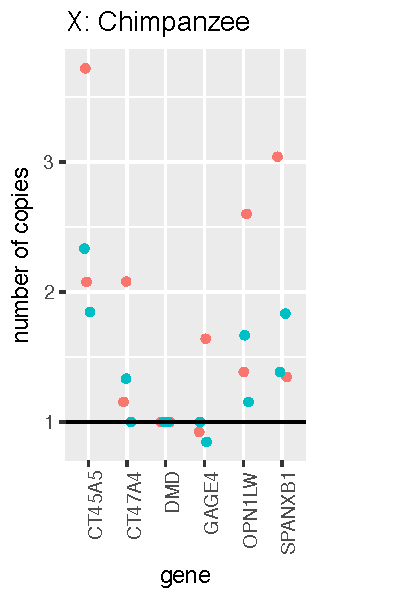
\includegraphics[height=\restrip\linewidth]{illustrations/X_species_chimp.pdf}\quad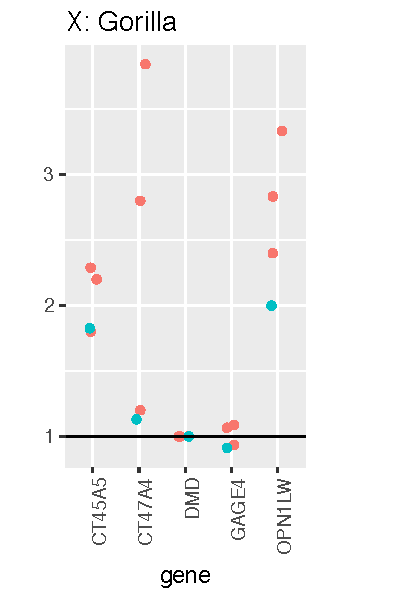
\includegraphics[height=\restrip\linewidth]{illustrations/X_species_gorilla.pdf}\quad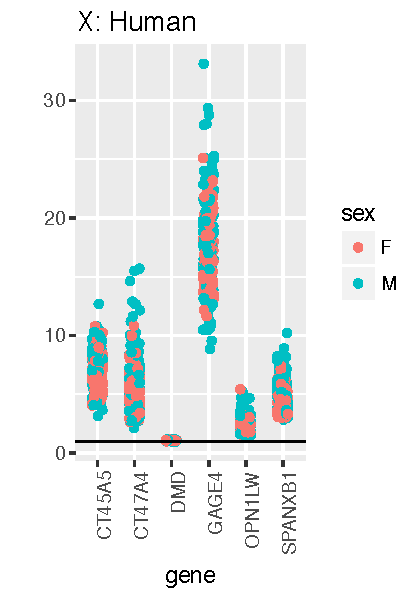
\includegraphics[height=\restrip\linewidth]{illustrations/X_human.pdf}
        \caption{X chromosome thingy}
        \label{fig:X_chrom_all}
    \end{figure}
\end{center}


\subsection{Y chromosome}
\begin{center}
    \begin{figure}
        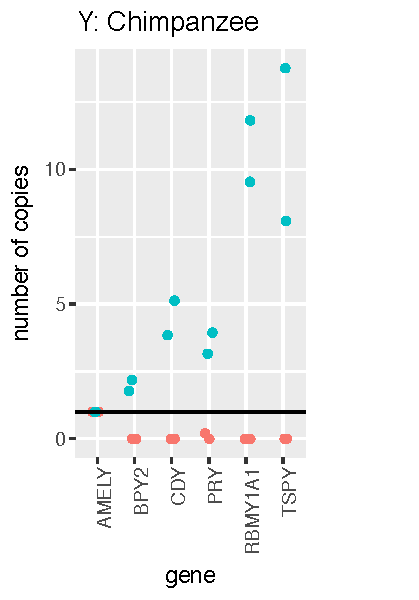
\includegraphics[height=\restrip\linewidth]{illustrations/Y_species_chimp.pdf}\quad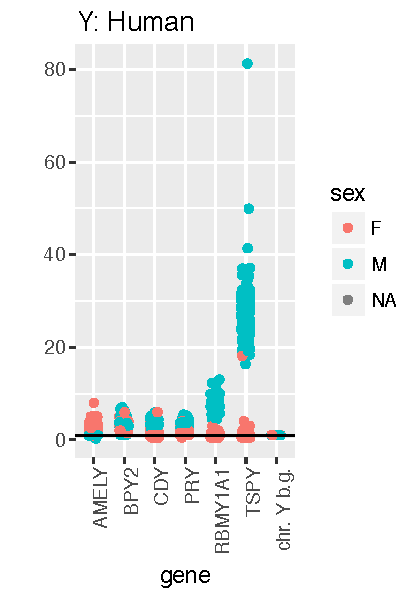
\includegraphics[height=\restrip\linewidth]{illustrations/Y_human.pdf}
        % consider removing sex == NA
        \caption{Y chromosome thingy}
        \label{fig:Y_chrom_all}
    \end{figure}
\end{center}





\begin{scheme}
  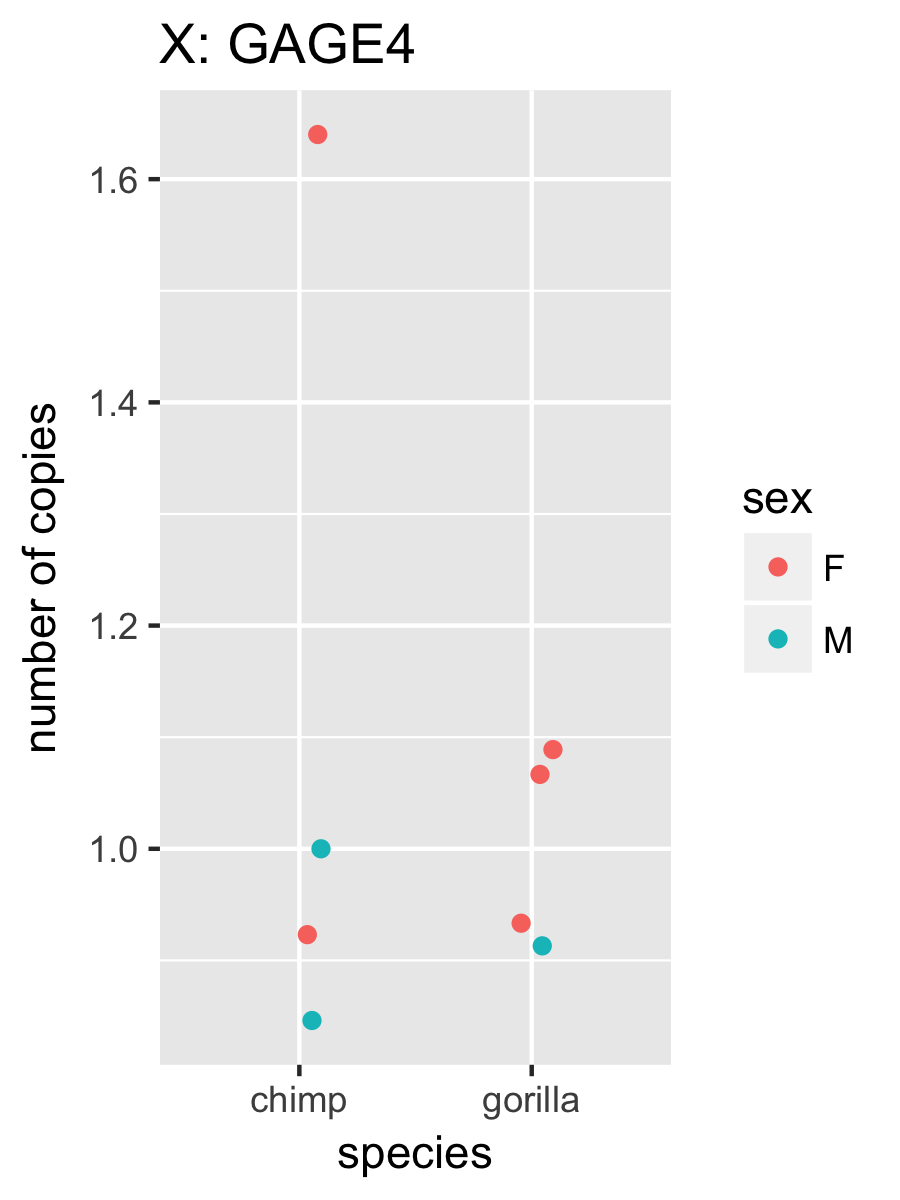
\includegraphics[height=10cm]{figure_X_gene_GAGE4.png}
  \caption{An example graphics}
  \label{sch:example}
\end{scheme}
%Optima for headings.
%Arial for everything else.

\subsection{Visual overview}
Placeholder
New float types are automatically set up by the class file. The
means graphics are included as follows (scheme \ref{sch:example}).  As
illustrated, the float is ``here'' if possible.
\begin{scheme}
  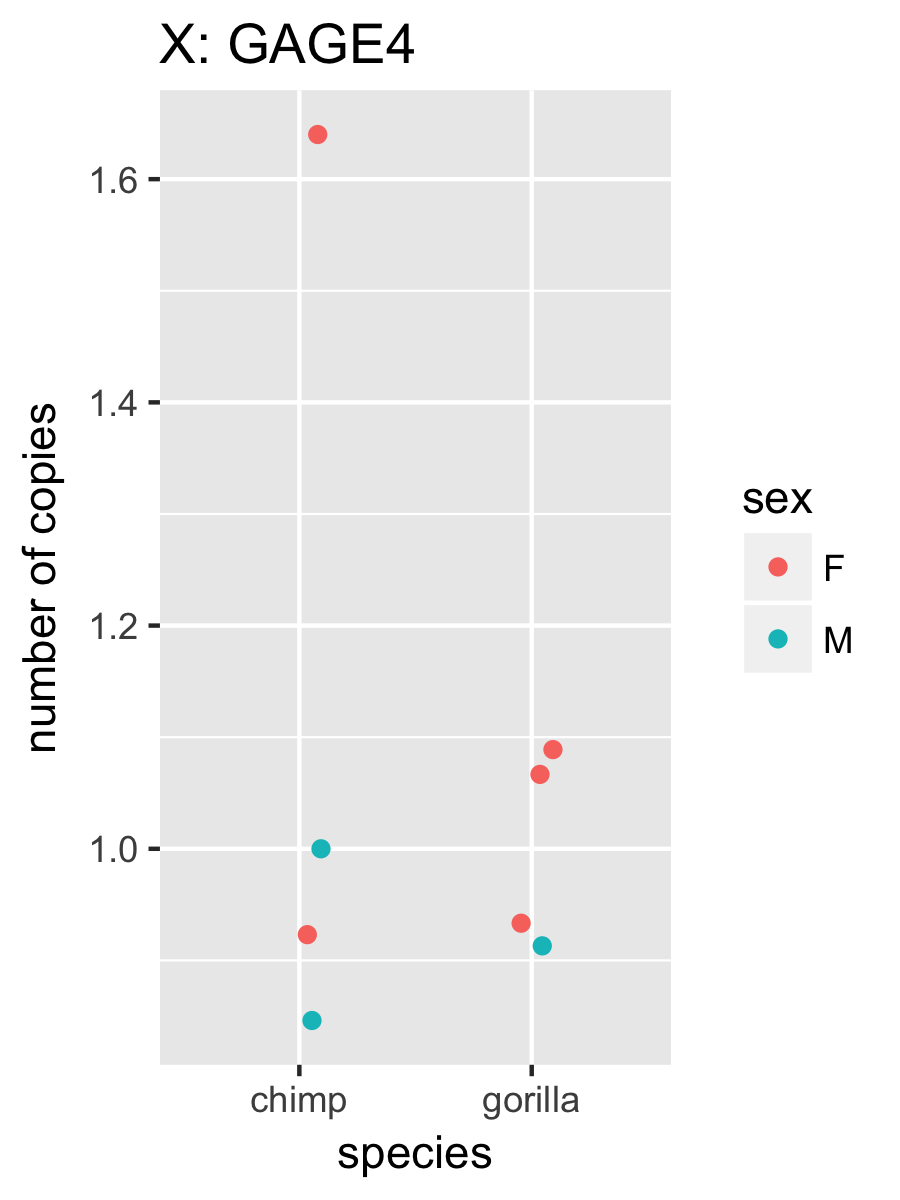
\includegraphics[height=10cm]{figure_X_gene_GAGE4.png}
  \caption{An example graphics}
  \label{sch:example}
\end{scheme}


\clearpage
%%%%%%%%%%%%%%%%%%%%%%%%%%%%%%%%%%%%%%%%%%%%%%%%%%%%% Discussion
\section{Discussion}

\subsection{Method criticism}
We only looked at genes that where ampliconic in human, and not the other way around. I mean, there should be genes with ampliconic behaviour in chimpanzee and gorilla, without ampliconicness in human.
I shouldn't have named the blasted gene results the name of the original, as I'm not just like creating my own annotation or whatever.

\subsection{Results criticisms) 
We didn't look at how ampliconic-ness relates to expression levels.
When are the genes expressed (in meiosis)?
For some reason, the gorilla Y chromosome was just too divergent. (No orthologs ?!)
It could be interesting to compare the paralogs between X and Y, to see which became ampliconic. (Maybe not so interesting because very few genes are present on the Y anyway)
Do the copies stay similar because there is a mechanism keeping them alike, or is it simply because the duplication event is too recent for any divergence to have happened?
How much different are the results when using the somewhat different human artificial chromosomes? This part should probably be in the beginning as it its outcome will change the results fro the species specific artificial chromosomes significantly.




% references
\bibliography{sample}

\end{document}
